\documentclass[11pt]{article}
\usepackage{tikz}
\usepackage{amssymb}
\usepackage{geometry}
\geometry{letterpaper, landscape, margin=0.4in}
\usetikzlibrary{positioning, calc}

% Door macros
\newcommand{\hdoor}[2]{%
  \fill[white,draw=black,thick] ({#1-0.1},{#2-0.12}) rectangle ({#1+0.1},{#2+0.12});%
}
\newcommand{\vdoor}[2]{%
  \fill[white,draw=black,thick] ({#1-0.12},{#2-0.1}) rectangle ({#1+0.12},{#2+0.1});%
}

\begin{document}

\begin{center}
{\Huge \textbf{THE GRAIN MOTHER'S RUIN}}\\[0.3em]
{\Large Level 1 --- The Ruined Temple | 33 Keyed Areas}
\end{center}

\vspace{0.3em}

\begin{center}
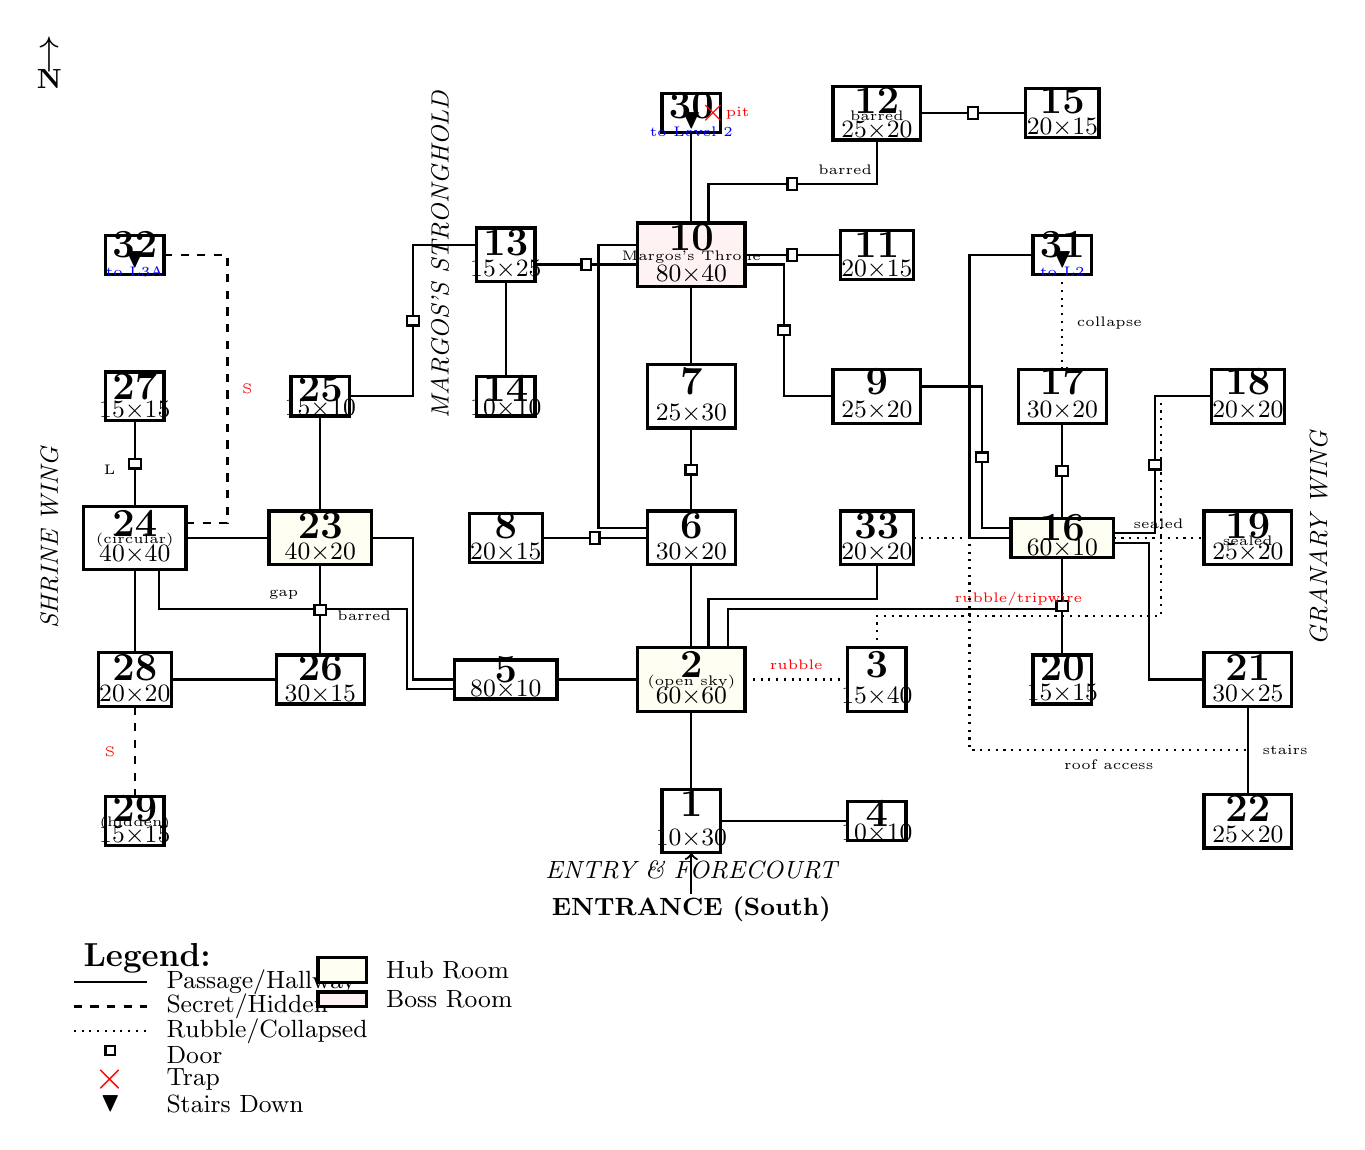
\begin{tikzpicture}[
    room/.style={draw, very thick, rectangle},
    hub/.style={draw, very thick, rectangle, fill=yellow!5},
    boss/.style={draw, very thick, rectangle, fill=red!5},
    connection/.style={draw, thick},
    secret/.style={dashed, thick},
    trap/.style={red},
    scale=0.62
]

% ============================================================
% Grid: 7 cols x 6 rows | CellW=2.5, CellH=1.6, Gutter=1.3
% Col centers: c0=1.25, c1=5.05, c2=8.85, c3=12.65, c4=16.45, c5=20.25, c6=24.05
% Row centers: r0=0.8, r1=3.7, r2=6.6, r3=9.5, r4=12.4, r5=15.3
% Vert gutters: g01=3.15, g12=6.95, g23=10.75, g34=14.55, g45=18.35, g56=22.15
% Horiz gutters: g01=2.25, g12=5.15, g23=8.05, g34=10.95, g45=13.85
% ============================================================

% ============================================================
% NORTH ARROW
% ============================================================
\node at (-0.5,16.5) {\Large $\uparrow$};
\node at (-0.5,16.0) {\textbf{N}};

% ENTRANCE label
\node[font=\small\bfseries] at (12.65,-1.0) {ENTRANCE (South)};
\draw[->, thick] (12.65,-0.7) -- (12.65,0.15);

% ============================================================
% ZONE: ENTRY \& FORECOURT (Rooms 1--5)
% Grid region: cols 2--4, rows 0--1
% ============================================================

% Room 1: The Broken Gate (10x30 ft)
% Cell: (3,0) -> center (12.65, 0.8)
\draw[room] (12.05,0.15) rectangle (13.25,1.45);
\node at (12.65,1.15) {\Large \textbf{1}};
\node[font=\small] at (12.65,0.45) {10$\times$30};

% Room 2: The Overgrown Courtyard (60x60 ft) -- central hub
% Cell: (3,1) -> center (12.65, 3.7)
\draw[hub] (11.55,3.05) rectangle (13.75,4.35);
\node at (12.65,4.0) {\Large \textbf{2}};
\node[font=\small] at (12.65,3.35) {60$\times$60};
\node[font=\tiny] at (12.65,3.65) {(open sky)};

% Room 3: The Collapsed Portico (15x40 ft)
% Cell: (4,1) -> center (16.45, 3.7)
\draw[room] (15.85,3.05) rectangle (17.05,4.35);
\node at (16.45,4.0) {\Large \textbf{3}};
\node[font=\small] at (16.45,3.35) {15$\times$40};

% Room 4: The Gatehouse Alcove (10x10 ft)
% Cell: (4,0) -> center (16.45, 0.8)
\draw[room] (15.85,0.4) rectangle (17.05,1.2);
\node at (16.45,0.95) {\Large \textbf{4}};
\node[font=\small] at (16.45,0.55) {10$\times$10};

% Room 5: The Colonnade (80x10 ft)
% Cell: (2,1) -> center (8.85, 3.7)
\draw[room] (7.8,3.3) rectangle (9.9,4.1);
\node at (8.85,3.9) {\Large \textbf{5}};
\node[font=\small] at (8.85,3.5) {80$\times$10};

% ============================================================
% ZONE: MARGOS'S STRONGHOLD (Rooms 6--15)
% Grid region: cols 2--4, rows 2--5
% ============================================================

% Room 6: The Antechamber (30x20 ft)
% Cell: (3,2) -> center (12.65, 6.6)
\draw[room] (11.75,6.05) rectangle (13.55,7.15);
\node at (12.65,6.85) {\Large \textbf{6}};
\node[font=\small] at (12.65,6.3) {30$\times$20};

% Room 7: The Goblin Warren (25x30 ft)
% Cell: (3,3) -> center (12.65, 9.5)
\draw[room] (11.75,8.85) rectangle (13.55,10.15);
\node at (12.65,9.8) {\Large \textbf{7}};
\node[font=\small] at (12.65,9.15) {25$\times$30};

% Room 8: The Crude Kitchen (20x15 ft)
% Cell: (2,2) -> center (8.85, 6.6)
\draw[room] (8.1,6.1) rectangle (9.6,7.1);
\node at (8.85,6.85) {\Large \textbf{8}};
\node[font=\small] at (8.85,6.3) {20$\times$15};

% Room 9: Orc Barracks (25x20 ft)
% Cell: (4,3) -> center (16.45, 9.5)
\draw[room] (15.55,8.95) rectangle (17.35,10.05);
\node at (16.45,9.8) {\Large \textbf{9}};
\node[font=\small] at (16.45,9.2) {25$\times$20};

% Room 10: The Great Hall (80x40 ft) -- Margos's Throne
% Cell: (3,4) -> center (12.65, 12.4)
\draw[boss] (11.55,11.75) rectangle (13.75,13.05);
\node at (12.65,12.75) {\Large \textbf{10}};
\node[font=\small] at (12.65,12.0) {80$\times$40};
\node[font=\tiny] at (12.65,12.35) {Margos's Throne};

% Room 11: The Bear Pit (20x15 ft)
% Cell: (4,4) -> center (16.45, 12.4)
\draw[room] (15.7,11.9) rectangle (17.2,12.9);
\node at (16.45,12.6) {\Large \textbf{11}};
\node[font=\small] at (16.45,12.1) {20$\times$15};

% Room 12: Margos's Private Quarters (25x20 ft)
% Cell: (4,5) -> center (16.45, 15.3)
\draw[room] (15.55,14.75) rectangle (17.35,15.85);
\node at (16.45,15.55) {\Large \textbf{12}};
\node[font=\small] at (16.45,14.95) {25$\times$20};
\node[font=\tiny] at (16.45,15.25) {barred};

% Room 13: The Trophy Room (15x25 ft)
% Cell: (2,4) -> center (8.85, 12.4)
\draw[room] (8.25,11.85) rectangle (9.45,12.95);
\node at (8.85,12.65) {\Large \textbf{13}};
\node[font=\small] at (8.85,12.1) {15$\times$25};

% Room 14: The Latrine Pit (10x10 ft)
% Cell: (2,3) -> center (8.85, 9.5)
\draw[room] (8.25,9.1) rectangle (9.45,9.9);
\node at (8.85,9.65) {\Large \textbf{14}};
\node[font=\small] at (8.85,9.25) {10$\times$10};

% Room 15: The Prison (20x15 ft)
% Cell: (5,5) -> center (20.25, 15.3)
\draw[room] (19.5,14.8) rectangle (21.0,15.8);
\node at (20.25,15.55) {\Large \textbf{15}};
\node[font=\small] at (20.25,15.0) {20$\times$15};

% ============================================================
% ZONE: THE GRANARY WING (Rooms 16--22)
% Grid region: cols 5--6, rows 0--3
% ============================================================

% Room 16: The Granary Corridor (60x10 ft)
% Cell: (5,2) -> center (20.25, 6.6)
\draw[hub] (19.2,6.2) rectangle (21.3,7.0);
\node at (20.25,6.8) {\Large \textbf{16}};
\node[font=\small] at (20.25,6.38) {60$\times$10};

% Room 17: Spoiled Grain Store (30x20 ft)
% Cell: (5,3) -> center (20.25, 9.5)
\draw[room] (19.35,8.95) rectangle (21.15,10.05);
\node at (20.25,9.8) {\Large \textbf{17}};
\node[font=\small] at (20.25,9.2) {30$\times$20};

% Room 18: The Collapsed Store (20x20 ft)
% Cell: (6,3) -> center (24.05, 9.5)
\draw[room] (23.3,8.95) rectangle (24.8,10.05);
\node at (24.05,9.8) {\Large \textbf{18}};
\node[font=\small] at (24.05,9.2) {20$\times$20};

% Room 19: The Sealed Granary (25x20 ft)
% Cell: (6,2) -> center (24.05, 6.6)
\draw[room] (23.15,6.05) rectangle (24.95,7.15);
\node at (24.05,6.85) {\Large \textbf{19}};
\node[font=\small] at (24.05,6.3) {25$\times$20};
\node[font=\tiny] at (24.05,6.55) {sealed};

% Room 20: The Grain-Master's Office (15x15 ft)
% Cell: (5,1) -> center (20.25, 3.7)
\draw[room] (19.65,3.2) rectangle (20.85,4.2);
\node at (20.25,3.95) {\Large \textbf{20}};
\node[font=\small] at (20.25,3.42) {15$\times$15};

% Room 21: The Old Millroom (30x25 ft)
% Cell: (6,1) -> center (24.05, 3.7)
\draw[room] (23.15,3.15) rectangle (24.95,4.25);
\node at (24.05,3.95) {\Large \textbf{21}};
\node[font=\small] at (24.05,3.4) {30$\times$25};

% Room 22: The Fermentation Cellar (25x20 ft)
% Cell: (6,0) -> center (24.05, 0.8)
\draw[room] (23.15,0.25) rectangle (24.95,1.35);
\node at (24.05,1.05) {\Large \textbf{22}};
\node[font=\small] at (24.05,0.5) {25$\times$20};

% ============================================================
% ZONE: THE SHRINE WING (Rooms 23--29)
% Grid region: cols 0--1, rows 0--3
% ============================================================

% Room 23: The Hall of Offerings (40x20 ft)
% Cell: (1,2) -> center (5.05, 6.6)
\draw[hub] (4.0,6.05) rectangle (6.1,7.15);
\node at (5.05,6.85) {\Large \textbf{23}};
\node[font=\small] at (5.05,6.3) {40$\times$20};

% Room 24: The Defiled Altar Room (40' diam circular)
% Cell: (0,2) -> center (1.25, 6.6)
\draw[room] (0.2,5.95) rectangle (2.3,7.25);
\node at (1.25,6.9) {\Large \textbf{24}};
\node[font=\small] at (1.25,6.25) {40$\times$40};
\node[font=\tiny] at (1.25,6.55) {(circular)};

% Room 25: The Vestry (15x10 ft)
% Cell: (1,3) -> center (5.05, 9.5)
\draw[room] (4.45,9.1) rectangle (5.65,9.9);
\node at (5.05,9.65) {\Large \textbf{25}};
\node[font=\small] at (5.05,9.25) {15$\times$10};

% Room 26: The Crypt of the Faithful (30x15 ft)
% Cell: (1,1) -> center (5.05, 3.7)
\draw[room] (4.15,3.2) rectangle (5.95,4.2);
\node at (5.05,3.95) {\Large \textbf{26}};
\node[font=\small] at (5.05,3.4) {30$\times$15};

% Room 27: The Reliquary (15x15 ft, octagonal)
% Cell: (0,3) -> center (1.25, 9.5)
\draw[room] (0.65,9.0) rectangle (1.85,10.0);
\node at (1.25,9.7) {\Large \textbf{27}};
\node[font=\small] at (1.25,9.2) {15$\times$15};

% Room 28: The Ossuary (20x20 ft)
% Cell: (0,1) -> center (1.25, 3.7)
\draw[room] (0.5,3.15) rectangle (2.0,4.25);
\node at (1.25,3.95) {\Large \textbf{28}};
\node[font=\small] at (1.25,3.4) {20$\times$20};

% Room 29: Mother Galvikta's Hidden Shrine (15x15 ft)
% Cell: (0,0) -> center (1.25, 0.8)
\draw[room] (0.65,0.3) rectangle (1.85,1.3);
\node at (1.25,1.05) {\Large \textbf{29}};
\node[font=\small] at (1.25,0.5) {15$\times$15};
\node[font=\tiny] at (1.25,0.75) {(hidden)};

% ============================================================
% ZONE: DESCENT POINTS (Rooms 30--33)
% ============================================================

% Room 30: The Grand Staircase (descending)
% Cell: (3,5) -> center (12.65, 15.3)
\draw[room] (12.05,14.9) rectangle (13.25,15.7);
\node at (12.65,15.45) {\Large \textbf{30}};
\node at (12.65,15.15) {$\blacktriangledown$};
\node[font=\tiny,blue] at (12.65,14.92) {to Level 2};

% Room 31: The Collapsed Passage (hole to Level 2)
% Cell: (5,4) -> center (20.25, 12.4)
\draw[room] (19.65,12.0) rectangle (20.85,12.8);
\node at (20.25,12.6) {\Large \textbf{31}};
\node at (20.25,12.3) {$\blacktriangledown$};
\node[font=\tiny,blue] at (20.25,12.05) {to L2};

% Room 32: The Sealed Shrine (secret spiral stairs to Level 3A)
% Cell: (0,4) -> center (1.25, 12.4)
\draw[room] (0.65,12.0) rectangle (1.85,12.8);
\node at (1.25,12.6) {\Large \textbf{32}};
\node at (1.25,12.3) {$\blacktriangledown$};
\node[font=\tiny,blue] at (1.25,12.05) {to L3A};

% Room 33: The Watchtower Ruin (20x20 ft)
% Cell: (4,2) -> center (16.45, 6.6)
\draw[room] (15.7,6.05) rectangle (17.2,7.15);
\node at (16.45,6.85) {\Large \textbf{33}};
\node[font=\small] at (16.45,6.3) {20$\times$20};

% Trap marker for Room 30 (pit trap on staircase)
\node[red] at (13.1,15.3) {\large $\times$};
\node[font=\tiny,red] at (13.6,15.3) {pit};

% ============================================================
% CONNECTIONS
% ============================================================

% --- ENTRY & FORECOURT CONNECTIONS ---

% Room 1 -> Room 2 (open passage north)
% Direct: same col (3), adjacent rows (0->1)
\draw[thick] (12.65,1.45) -- (12.65,3.05);

% Room 1 -> Room 4 (open archway east)
% Direct: same row (0), adjacent cols (3->4)
\draw[thick] (13.25,0.8) -- (15.85,0.8);

% Room 2 -> Room 3 (rubble passage east)
% Direct: same row (1), adjacent cols (3->4)
\draw[thick,dotted] (13.75,3.7) -- (15.85,3.7);
\node[above,font=\tiny,red] at (14.8,3.7) {rubble};

% Room 2 -> Room 5 (open passage west)
% Direct: same row (1), adjacent cols (3->2)
\draw[thick] (11.55,3.7) -- (9.9,3.7);

% Room 2 -> Room 6 (passage north)
% Direct: same col (3), adjacent rows (1->2)
\draw[thick] (12.65,4.35) -- (12.65,6.05);

% Room 2 -> Room 16 (passage east to Granary)
% L-route: exit 2 top-right -> gutter row 1-2 -> right -> down to 16
\draw[thick] (13.4,4.35) -- (13.4,5.15) -- (20.25,5.15) -- (20.25,6.2);

% Room 2 -> Room 33 (crumbling stair northeast)
% L-route: exit 2 top -> gutter row 1-2 -> right -> up to 33
\draw[thick] (13.0,4.35) -- (13.0,5.35) -- (16.45,5.35) -- (16.45,6.05);

% --- COLONNADE TO SHRINE WING ---

% Room 5 -> Room 23 (open passage, north end of colonnade)
% L-route: exit 5 left -> gutter col 1-2 -> up -> right to 23
\draw[thick] (7.8,3.7) -- (6.95,3.7) -- (6.95,6.6) -- (6.1,6.6);

% Room 5 -> Room 24 (gap in wall, halfway along colonnade)
% Multi-turn: exit 5 left -> gutter col 1-2 -> gutter row 1-2 -> left -> up to 24
\draw[thick] (7.8,3.5) -- (6.83,3.5) -- (6.83,5.15) -- (1.75,5.15) -- (1.75,5.95);
\node[above,font=\tiny] at (4.3,5.15) {gap};

% --- MARGOS'S STRONGHOLD CONNECTIONS ---

% Room 6 -> Room 7 (door north)
% Direct: same col (3), adjacent rows (2->3)
\draw[thick] (12.65,7.15) -- (12.65,8.85);
\vdoor{12.65}{8.0}

% Room 6 -> Room 8 (door west)
% Direct: same row (2), adjacent cols (3->2)
\draw[thick] (11.75,6.6) -- (9.6,6.6);
\hdoor{10.67}{6.6}

% Room 6 -> Room 10 (passage north, routes around Room 7)
% L-route: exit 6 left -> gutter col 2-3 -> up -> right to 10 left
\draw[thick] (11.75,6.8) -- (10.75,6.8) -- (10.75,12.6) -- (11.55,12.6);

% Room 7 -> Room 10 (passage north/east)
% Direct: same col (3), adjacent rows (3->4)
\draw[thick] (12.65,10.15) -- (12.65,11.75);

% Room 9 -> Room 10 (door west)
% L-route: exit 9 left -> gutter col 3-4 -> up -> right to 10 right
\draw[thick] (15.55,9.5) -- (14.55,9.5) -- (14.55,12.2) -- (13.75,12.2);
\vdoor{14.55}{10.85}

% Room 10 -> Room 11 (iron door east)
% Direct: same row (4), adjacent cols (3->4)
\draw[thick] (13.75,12.4) -- (15.7,12.4);
\hdoor{14.72}{12.4}

% Room 10 -> Room 12 (barred door, north-east)
% L-route: exit 10 top -> gutter row 4-5 -> right -> down to 12
\draw[thick] (13.0,13.05) -- (13.0,13.85) -- (16.45,13.85) -- (16.45,14.75);
\hdoor{14.72}{13.85}
\node[above,font=\tiny] at (15.8,13.85) {barred};

% Room 10 -> Room 13 (door west)
% Direct: same row (4), adjacent cols (3->2)
\draw[thick] (11.55,12.2) -- (9.45,12.2);
\hdoor{10.5}{12.2}

% Room 10 -> Room 30 (passage north to Grand Staircase)
% Direct: same col (3), adjacent rows (4->5)
\draw[thick] (12.65,13.05) -- (12.65,14.9);

% Room 12 -> Room 15 (door east)
% Direct: same row (5), adjacent cols (4->5)
\draw[thick] (17.35,15.3) -- (19.5,15.3);
\hdoor{18.42}{15.3}

% Room 13 -> Room 14 (open archway south)
% Direct: same col (2), adjacent rows (4->3)
\draw[thick] (8.85,11.85) -- (8.85,9.9);

% Room 16 -> Room 9 (hallway west)
% L-route: exit 16 left -> gutter col 4-5 -> up -> left to 9 right
\draw[thick] (19.2,6.8) -- (18.6,6.8) -- (18.6,9.7) -- (17.35,9.7);
\vdoor{18.6}{8.25}

% --- GRANARY WING CONNECTIONS ---

% Room 16 -> Room 17 (door north)
% Direct: same col (5), adjacent rows (2->3)
\draw[thick] (20.25,7.0) -- (20.25,8.95);
\vdoor{20.25}{7.97}

% Room 16 -> Room 18 (door, NE to Collapsed Store)
% L-route: exit 16 right -> gutter col 5-6 -> up -> right to 18
\draw[thick] (21.3,6.7) -- (22.15,6.7) -- (22.15,9.5) -- (23.3,9.5);
\vdoor{22.15}{8.1}

% Room 16 -> Room 19 (sealed door east)
% Direct: same row (2), adjacent cols (5->6)
\draw[thick,dotted] (21.3,6.6) -- (23.15,6.6);
\node[above,font=\tiny] at (22.22,6.6) {sealed};

% Room 16 -> Room 20 (door south)
% Direct: same col (5), adjacent rows (2->1)
\draw[thick] (20.25,6.2) -- (20.25,4.2);
\vdoor{20.25}{5.2}

% Room 16 -> Room 21 (passage SE to Millroom)
% L-route: exit 16 right -> gutter col 5-6 -> down -> right to 21
\draw[thick] (21.3,6.5) -- (22.03,6.5) -- (22.03,3.7) -- (23.15,3.7);

% Room 16 -> Room 31 (passage SE, routes around Room 17)
% L-route: exit 16 left -> gutter col 4-5 -> up -> right to 31
\draw[thick] (19.2,6.6) -- (18.35,6.6) -- (18.35,12.4) -- (19.65,12.4);

% Room 17 -> Room 31 (collapsed floor)
% Direct: same col (5), adjacent rows (3->4)
\draw[thick,dotted] (20.25,10.05) -- (20.25,12.0);
\node[right,font=\tiny] at (20.35,11.0) {collapse};

% Room 21 -> Room 22 (stairs down south)
% Direct: same col (6), adjacent rows (1->0)
\draw[thick] (24.05,3.15) -- (24.05,1.35);
\node[right,font=\tiny] at (24.15,2.25) {stairs};

% Room 3 -> Room 18 (rubble passage, alternate route)
% Multi-turn: exit 3 top -> gutter row 1-2 -> right -> gutter col 5-6 -> up -> right to 18
\draw[thick,dotted] (16.45,4.35) -- (16.45,5.0) -- (22.27,5.0) -- (22.27,9.5) -- (23.3,9.5);
\node[above,font=\tiny,red] at (19.35,5.0) {rubble/tripwire};

% Room 33 -> Room 21 (collapsed roof access, alternate entry)
% Multi-turn: exit 33 right -> gutter col 4-5 -> down -> gutter row 0-1 -> right -> up to 21
\draw[thick,dotted] (17.2,6.6) -- (18.35,6.6) -- (18.35,2.25) -- (24.05,2.25) -- (24.05,3.15);
\node[below,font=\tiny] at (21.2,2.25) {roof access};

% Room 25 -> Room 13 (hallway east)
% L-route: exit 25 right -> gutter col 1-2 -> up -> right to 13 left
\draw[thick] (5.65,9.5) -- (6.95,9.5) -- (6.95,12.6) -- (8.25,12.6);
\vdoor{6.95}{11.05}

% --- SHRINE WING CONNECTIONS ---

% Room 23 -> Room 24 (open arch west)
% Direct: same row (2), adjacent cols (1->0)
\draw[thick] (4.0,6.6) -- (2.3,6.6);

% Room 23 -> Room 25 (open passage north/up)
% Direct: same col (1), adjacent rows (2->3)
\draw[thick] (5.05,7.15) -- (5.05,9.1);

% Room 23 -> Room 26 (barred iron door south)
% Direct: same col (1), adjacent rows (2->1)
\draw[thick] (5.05,6.05) -- (5.05,4.2);
\vdoor{5.05}{5.12}
\node[right,font=\tiny] at (5.2,5.0) {barred};

% Room 24 -> Room 27 (locked door west/up)
% Direct: same col (0), adjacent rows (2->3)
\draw[thick] (1.25,7.25) -- (1.25,9.0);
\vdoor{1.25}{8.12}
\node[left,font=\tiny] at (1.05,8.0) {L};

% Room 24 -> Room 28 (passage south/down)
% Direct: same col (0), adjacent rows (2->1)
\draw[thick] (1.25,5.95) -- (1.25,4.25);

% Room 24 -> Room 32 (secret door north, routes around Room 27)
% L-route: exit 24 right -> gutter col 0-1 -> up -> left to 32
\draw[thick,dashed] (2.3,6.9) -- (3.15,6.9) -- (3.15,12.4) -- (1.85,12.4);
\node[right,font=\tiny,red] at (3.25,9.65) {S};

% Room 26 -> Room 28 (passage west)
% Direct: same row (1), adjacent cols (1->0)
\draw[thick] (4.15,3.7) -- (2.0,3.7);

% Room 28 -> Room 29 (secret passage south)
% Direct: same col (0), adjacent rows (1->0)
\draw[thick,dashed] (1.25,3.15) -- (1.25,1.3);
\node[left,font=\tiny,red] at (1.05,2.22) {S};

% ============================================================
% LEGEND
% ============================================================
\node[anchor=west,font=\large] at (0.0,-2.0) {\textbf{Legend:}};

\draw[thick] (0.0,-2.5) -- (1.5,-2.5);
\node[anchor=west,font=\small] at (1.7,-2.5) {Passage/Hallway};

\draw[thick,dashed] (0.0,-3.0) -- (1.5,-3.0);
\node[anchor=west,font=\small] at (1.7,-3.0) {Secret/Hidden};

\draw[thick,dotted] (0.0,-3.5) -- (1.5,-3.5);
\node[anchor=west,font=\small] at (1.7,-3.5) {Rubble/Collapsed};

\fill[white,draw=black,thick] (0.65,-4.0) rectangle (0.85,-3.8);
\node[anchor=west,font=\small] at (1.7,-4.0) {Door};

\node[red] at (0.75,-4.5) {\Large $\times$};
\node[anchor=west,font=\small] at (1.7,-4.5) {Trap};

\node at (0.75,-5.0) {$\blacktriangledown$};
\node[anchor=west,font=\small] at (1.7,-5.0) {Stairs Down};

\draw[very thick, fill=yellow!5] (5.0,-2.5) rectangle (6.0,-2.0);
\node[anchor=west,font=\small] at (6.2,-2.25) {Hub Room};

\draw[very thick, fill=red!5] (5.0,-3.0) rectangle (6.0,-2.7);
\node[anchor=west,font=\small] at (6.2,-2.85) {Boss Room};

% ============================================================
% ZONE LABELS
% ============================================================
\node[font=\small\itshape] at (12.65,-0.2) {ENTRY \& FORECOURT};
\node[font=\small\itshape, rotate=90] at (7.5,12.4) {MARGOS'S STRONGHOLD};
\node[font=\small\itshape, rotate=90] at (25.5,6.6) {GRANARY WING};
\node[font=\small\itshape, rotate=90] at (-0.5,6.6) {SHRINE WING};

\end{tikzpicture}
\end{center}

\vspace{0.5em}

\section*{Room Key}
\begin{small}
\begin{tabular}{rl|rl|rl}
1 & Broken Gate (10$\times$30) & 12 & Margos's Quarters (25$\times$20) & 23 & Hall of Offerings (40$\times$20) \\
2 & Overgrown Courtyard (60$\times$60) & 13 & Trophy Room (15$\times$25) & 24 & Defiled Altar Room (40 circ.) \\
3 & Collapsed Portico (15$\times$40) & 14 & Latrine Pit (10$\times$10) & 25 & Vestry (15$\times$10) \\
4 & Gatehouse Alcove (10$\times$10) & 15 & Prison (20$\times$15) & 26 & Crypt of the Faithful (30$\times$15) \\
5 & Colonnade (80$\times$10) & 16 & Granary Corridor (60$\times$10) & 27 & Reliquary (15$\times$15, locked) \\
6 & Antechamber (30$\times$20) & 17 & Spoiled Grain Store (30$\times$20) & 28 & Ossuary (20$\times$20) \\
7 & Goblin Warren (25$\times$30) & 18 & Collapsed Store (20$\times$20) & 29 & Galvikta's Shrine (15$\times$15) \\
8 & Crude Kitchen (20$\times$15) & 19 & Sealed Granary (25$\times$20) & 30 & Grand Staircase $\rightarrow$ L2 \\
9 & Orc Barracks (25$\times$20) & 20 & Grain-Master's Office (15$\times$15) & 31 & Collapsed Passage $\rightarrow$ L2 \\
10 & Great Hall (80$\times$40) & 21 & Old Millroom (30$\times$25) & 32 & Sealed Shrine $\rightarrow$ L3A \\
11 & Bear Pit (20$\times$15) & 22 & Fermentation Cellar (25$\times$20) & 33 & Watchtower Ruin (20$\times$20) \\
\end{tabular}
\end{small}

\section*{Connections to Other Levels}
\begin{small}
\begin{itemize}
    \item \textbf{Room 30 (Grand Staircase):} Stairs down to Level 2 --- main descent, pit trap at switchback
    \item \textbf{Room 31 (Collapsed Passage):} Hidden hole down to Level 2 --- unstable, rat-infested
    \item \textbf{Room 32 (Sealed Shrine):} Secret spiral stairs to Level 3A --- bypasses Level 2 entirely
\end{itemize}
\end{small}

\end{document}
